\chapter{Introdução}

O termo Internet das Coisas, do inglês, \textit{Internet of Things} (IoT), foi usado pela primeira vez em 1998 para definir objetos do mundo físico representados virtualmente por meio de dispositivos interconectados~\cite{weber2010internet}. 

Advinda do avanço das áreas de sistemas embarcados, microeletrônica, comunicação e tecnologia de informações ~\cite{iot2016}, a IoT é considerada uma das mais promissoras tecnologias emergentes~\cite{gartner2015gartner}. Conforme o crescimento da quantidade de dispositivos e aplicativos conectados a \textit{Internet}, aumenta o interesse dos usuários em adquiri-los, tal como o de empresas em investir neste mercado~\cite{mukherjee2016ranking}.

Em estudo realizado pela \textit{Acquity Group}, mais de dois terços dos consumidores planejam comprar tecnologia conectada para suas casas até 2019~\cite{press2014internet}. Também, até 2017, 82\% das empresas implementarão a IoT de alguma forma, de acordo com relatório publicado pela \textit{Business Insider UK}~\cite{danova2014bi}.

Através da conexão e troca de mensagens entre os dispositivos, é possível realizar o monitoramento de ambientes controlados,  dispondo de uma vasta área de aplicações. Entre elas, pode-se destacar: carros, cidades e fazendas inteligentes; transporte e logística; cuidados médicos; interação pessoal e social; e processos industriais~\cite{sankarinternet, bandyopadhyay2011internet, atzori2010internet}.

Dentre os diversos fatores responsáveis pelo crescimento do interesse na área, ressalta-se a miniaturização do \textit{hardware}, além da criação do Protocolo de \textit{Internet} IPv6~\cite{press2014internet}. Capaz de alocar até $2^{128}$ endereços IP, o IPv6 possibilita a conexão de uma imensa quantidade de dispositivos~\cite{mukherjee2016ranking}.

Segundo a Cisco, até 2020 haverá cerca de 50 bilhões de dispositivos conectados, e até 2022, o mercado de soluções para IoT acrescentará em torno de 14,4 trilhões de dólares ao PIB global~\cite{morgan2014forbes}.

De forma geral, dispositivos utilizados em IoT possuem recursos limitados de memória e processamento, além de operarem em ambientes com baixa largura de banda ou redes instáveis ~\cite{weber2010internet, iot2016, suo2012security}. Portanto, é essencial que a comunicação e a troca de dados entre eles seja executada da forma eficiente, sendo este, um dos principais desafios enfrentados em IoT~\cite{bandyopadhyay2011internet, suo2012security}.

Devido as suas características, as aplicações de IoT necessitam de padronizações específicas. Logo, tratando-se estritamente da comunicação entre os dispositivos, foi desenvolvido em 1999 pela IBM e Eurotech o protocolo MQTT (\textit{Message Queue Telemetry Transport protocol})~\cite{mqttv3.1}. 

Padronizado em 2014 pela OASIS~\cite{mqttv3.1.1}, o MQTT tem como principal objetivo minimizar o uso de largura de banda da rede e recursos dos dispositivos. Para isso, o protocolo foi desenvolvido com base em diversos conceitos que asseguram uma alta taxa de entrega das mensagens~\cite{chen2014responsive}.

Com o advento do MQTT, suas propriedades e aplicações tornaram-se alvo de pesquisas, a fim de encontrar vulnerabilidades, ambiguidades e inconsistências, contribuindo com o aprimoramento da tecnologia~\cite{aziz2016formal, mladenov2017formal}.

Diversos métodos são utilizados por especialistas para verificação e validação de propriedades de protocolos e sistemas complexos, entre eles, destaca-se: simulação, teste de protótipo, verificação dedutiva e verificação formal~\cite{clarke1999model}. 

Com exceção da verificação formal, os demais métodos, embora sejam amplamente usados, não garantem total ausência de erros no funcionamento do sistema, uma vez que são incapazes de checar de forma automática todos os caminhos possíveis, visto que dependem de decisões humanas acerca de quais pontos devem ser analisados, tornando-os suscetíveis a falhas~\cite{clarke1999model}. 

Ademais, tais métodos apresentam deficiências que podem envolver tempo excessivo para análise e observação, além de gastos elevados com especialistas encarregados de aplicá-los~\cite{clarke1999model}.

A verificação formal engloba a técnica de teste baseado em modelo, também conhecida como \textit{Model Checking}, a qual proporciona uma série de vantagens em comparação com os outros métodos, tais como aplicação automática, verificação completa de todos os caminhos possíveis e produção de contraexemplos que demonstram quando uma dada propriedade não é satisfeita. Além disso, não é necessário a especificação completa do sistema, uma vez que seus módulos podem ser representados separadamente. Assim, pode-se verificar apenas os pontos críticos, poupando tempo e provendo maior segurança e confiabilidade~\cite{clarke1999model}.

Portanto, este trabalho tem como objetivo desenvolver um algoritmo para verificação formal da versão 3.1.1 do protoclo MQTT e suas propriedades por meio de \textit{Model Checking}.

O algoritmo será implementado e testado por meio de um estudo de caso. Com isso, espera-se que a comunicação entre dispositivos nos projetos de IoT que utilizam o protocolo MQTT possa ser verificada antes de sua implantação.

\section{Motivação}

Como dito anteriormente, a Internet das Coisas é uma das mais poderosas tecnologias emergentes, estima-se que até 2022 ela irá adicionar de 14,4 trilhões de dólares ao PIB global, e que em 2020 haverá em torno de 50 bilhões de dispositivos interconectados~\cite{morgan2014forbes}, aumentando a demanda por sensores, dispositivos de rede sem fio, serviços de armazenamento em nuvem, entre outros serviços e dispositivos que compõem este ambiente tecnológico, despertando assim, o interesse dos setores industriais e acadêmicos.

A comunicação é um fator crítico num projeto em IoT, pois a troca de dados e informações entre os dispositivos é essencial para seu sucesso. Com a heterogeneidade de dispositivos que compõem o ambiente, padronizações são necessárias para manter a interoperabilidade entre os mesmos, sendo essa uma das funções que os protocolos pretender cumprir.

O protocolo MQTT foi desenvolvido especialmente para aplicações em IoT e M2M (\textit{Machine-to-Machine}). Com um cabeçalho de apenas 2 \textit{bytes}, e implementando um servidor próprio, chamado de \textit{broker}, é capaz de prover a troca de mensagens entre dispositivo por meio da estratégia \textit{publish/subscribe}, minimizando o uso de banda de rede e recursos do dispositivo~\cite{mqttv3.1.1}. 

\begin{figure}[ht]
	\centering
	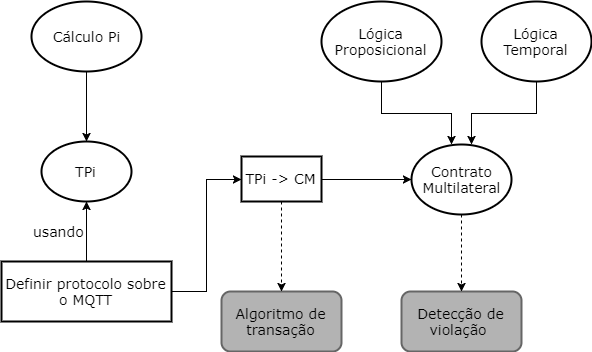
\includegraphics[width=1\textwidth]{imagens/tcc_estrutura.png}
	\caption{Escopo do método proposto.
		\label{fig:tcc_escopo}}
\end{figure}
\FloatBarrier

\section{Formulação e Escopo do Problema}

Como relatado acima, não se tem conhecimento de alguma ferramenta baseada em verificação formal que permita modelar a comunicação entre os dispositivos de projetos em IoT, assim como realizar a checagem automática de suas propriedades. Em vista disso, a principal questão a ser respondida é:

\textbf{É possível modelar e verificar a comunicação entre dispositivos que utilizam o protocolo MQTT?}

No intuito de responder essa questão, a resolução das seguintes subquestões devem ser fornecidas:

\textbf{\textit{(1) É possível modelar o MQTT?}}


No estudo desenvolvido por~\citeauthor{aziz2016formal}, e que serve de base para este trabalho, o protocolo é modelado através de uma álgebra temporal de processos, chamada \textit{TPi}.

\textbf{\textit{(2) É possível realizar a verificação formal do MQTT?}}

A partir do elaborado por~\citeauthor{aziz2016formal}, pode-se criar um algoritmo baseado em \textit{Model Checking} que faça a verificação de suas propriedades, o que leva ao objetivo do trabalho.

\section{Objetivos gerais e específicos}

